%%%%%%%%%%%%%%%%%%%%%%%%%%%%%%%%%%%%%%%%%%%%%%%%%%%%%%%%%
%% FINAL PAPER
%% Developer-Module Networks
%%
%% Authors: Bryan J Muscedere
%% Rafi Turas
%%%%%%%%%%%%%%%%%%%%%%%%%%%%%%%%%%%%%%%%%%%%%%%%%%%%%%%%%

\documentclass{sig-alternate-05-2015}
\usepackage{color}
\usepackage{multirow}
\usepackage{adjustbox}
\begin{document}

%%%%%%%%%%%%%%%%%%%%%%%%%%%%%%%%%%%%%%%%%%%%%%%%%%%%%%%%%
% Copyright Info
%%%%%%%%%%%%%%%%%%%%%%%%%%%%%%%%%%%%%%%%%%%%%%%%%%%%%%%%%
\setcopyright{acmcopyright}
\doi{10.475/123_4}
\isbn{123-4567-24-567/08/06}
\conferenceinfo{PLDI '13}{June 16--19, 2013, Seattle, WA, USA}
\acmPrice{\$15.00}
\conferenceinfo{WOODSTOCK}{'97 El Paso, Texas USA}

%%%%%%%%%%%%%%%%%%%%%%%%%%%%%%%%%%%%%%%%%%%%%%%%%%%%%%%%%
% Title and Authors
%%%%%%%%%%%%%%%%%%%%%%%%%%%%%%%%%%%%%%%%%%%%%%%%%%%%%%%%%
\title{Can Developer-Module Networks Predict Failures in Open-Source GitHub Projects?}

\numberofauthors{2}

\author{
\alignauthor
Bryan J. Muscedere\\
       \affaddr{University of Waterloo}\\
       \affaddr{200 University Ave W}\\
       \affaddr{Waterloo, Canada}\\
       \email{bmuscede@uwaterloo.ca}
\alignauthor
Rafi Turas\\
       \affaddr{University of Waterloo}\\
       \affaddr{200 University Ave W}\\
       \affaddr{Waterloo, Canada}\\
       \email{rsturas@uwaterloo.ca}
       }
\maketitle

%%%%%%%%%%%%%%%%%%%%%%%%%%%%%%%%%%%%%%%%%%%%%%%%%%%%%%%%%
% Abstract
%%%%%%%%%%%%%%%%%%%%%%%%%%%%%%%%%%%%%%%%%%%%%%%%%%%%%%%%%
\begin{abstract}
Early failure prediction through the use of internal project metrics remains an open area of software engineering research that has been subject to many different studies. Several previous studies have looked at code metrics, organizational metrics, and social networks for use as failure predictors in projects. One past study found that a type of social network known as developer-module networks can accurately predict failures in Windows Vista with a precision of 83\% and 89\%. While these results are encouraging, this study only examined Windows Vista when . This paper presents a study that tests whether developer-module networks can be valid predictors of failures for fifteen different open-source projects stored on GitHub. Results of our study show that, for the fifteen projects, \textit{bug-prone} files can be predicted with an average precision of 76\% and average recall of 76\%. Further, we present a software tool called \textbf{NetworkMine} that allows users to duplicate the methodology presented in this paper on any GitHub based project automatically.
\end{abstract}

%%%%%%%%%%%%%%%%%%%%%%%%%%%%%%%%%%%%%%%%%%%%%%%%%%%%%%%%%
% Introduction
%%%%%%%%%%%%%%%%%%%%%%%%%%%%%%%%%%%%%%%%%%%%%%%%%%%%%%%%%
\section{Introduction}
Software developers want to maximize the amount of time that they spend building new features and minimize the amount of time that they spend in performing quality assurance. Since buggy binaries and components can impact the release date of new products and the profit of software companies, it would be helpful to have reliable tools that narrow the search space for potentially buggy source files. The impact of bugs is even greater for large projects that have many source files. Much research has already focused on the development of tools and metrics that are able to identify software bugs early. However, in order to build such tools, researchers must investigate methods that identify failure-prone source files with high accuracy. 

Our study extends a previous study conducted at Microsoft Research by Pinzger et al, \cite{pingzer:networks} in 2008. Their study looks at failure-prediction metrics for prediction of bug-prone binaries in Windows Vista. The Windows Vista project is interesting since it is a large project consisting of approximately 3500 binaries and 3000 developers \cite{Bird:Distributed}. In the original study, the binary files, commit histories, and failure related data were collected and a developer-module network representing the interactions between developers and files was built. By constructing this graph for Vista, the researchers were able to calculate network centrality metrics for each of the binaries to determine how developers contributed to the binaries. By performing logistic regression on their contribution network, the researchers were able to predict failure-prone binaries with a precision of 83\% and recall of 89\%.

While the results from \cite{pingzer:networks} is extremely encouraging, their study only analyzes the closed-source project Windows Vista. Since the study is empirical in nature, there is a danger of extrapolating these results to be used in other software domains \cite{oram:software}. As such, developers that aim to use these results to predict failures in their projects may discover that the methodology used in \cite{pingzer:networks} does not produce the same results. This drawback is evident in many different studies that aim to provide failure-prediction for projects including \cite{Bird:Distributed} and \cite{Nag:Failures}.

Based on this underlying limitation, there is a motivation to duplicate many of these failure-prediction studies for projects in different domains to determine whether the identified metrics hold up across numerous projects. Recently, duplicating these studies across many different projects has become feasible through the advent of large code repositories such as GitHub and SurgeForge. Since GitHub is home to thousands of open-source projects, many different solutions and guidelines have been developed to mine it for project data \cite{Kalliamvakou:GitHub}.

This project aimed to validate the findings of Pinzger et al.'s study of developer-module networks on failure-prediction in Windows Vista by testing a collection of large open-source projects stored on GitHub. To do this, we built developer-module networks for each of the projects, computed network centrality metrics to determine how developers in each project interacted with files, and tested whether these metrics could be used to predict \textit{bug-prone} files. The following research questions were investigated throughout the duration of the project:
\\ \textbf{Research Question (RQ) \#1:} Is the network centrality of a file related to the number of commits and bug fixes of that file?
\\ \textbf{Research Question (RQ) \#2:} Can network centrality metrics be used as a valid predictor for defects?

The rest of this paper is organized as follows: Section \ref{background} describes the concepts of developer-module networks and network centrality metrics. Section \ref{study} describes the methodology of the study conducted in this paper. Section \ref{results} presents the results of the study. Section \ref{future_work} discusses further future areas of work.

\section{Background}
\label{background}
Before the methodology can be described, we describe previous work in the area of failure prediction and provide the formal definitions of developer-module networks and the network centralities used in this paper. Importantly, the attempt to use developer-module networks to predict failure-proneness is part of a long history of efforts to utilize organizational and process metrics to build better software instead of purely code based metrics.

\subsection{Related \& Previous Work}
Previous studies such as \cite{Nag:Org} have looked at using the organizational structure of a project's development to predict failures. Conway's Law states that the organizational structure of the team influences the organizational structure of the software and, with Conway's Corollary, if the structure of the software matches the structure of the team, it will lead to better quality of software \cite{oram:software}. As such, the study conducted in \cite{Nag:Org} found that through the use of organizational metrics, failures could be predicted in Windows Vista with a precision of 87\% and recall of 84\%. Thus, the structure of a piece of software will naturally tend to mirror the organization of the team that created it. While the results here were useful in establishing that software created by a team will automatically reflect its organizational structure, this study does not look at the interactions between files and developers in whole.

Since that paper was published there have been other studies that have looked at failures from an organizational perspective. In addition to the Pinzger e al. study \cite{pingzer:networks} which looked at contribution networks, a Microsoft study from 2009 \cite{Bird:Sociotechnical}, looked at a hybrid of contribution (developer-module) networks and dependency networks called sociotechnical networks. In the study, the authors tested their sociotechincal network on Windows Vista and five releases of Eclipse to predict failures. Overall, the authors found precision and recall values as high as 85\% across all of their studies. This project opted not to use these networks in the study due to their higher level of complexity and similar precision and recall values to those obtained from developer-module networks.

A major motivation behind performing this test on open-source projects is because, from open-source software research, process metrics have been found to be better failure predictors compared to code metrics \cite{rahman:metrics}. This provides encouragement that the results form the original Pinzger et al. study may also apply to open-source projects.

\subsection{Developer-Module Networks}
This study utilizes developer-module networks to represent the interactions between developers and files in a network. A type of social network, developer-module networks are special graphs of the form \(G = (D, F, E)\). In this, \(D\) and \(F\) are a set of nodes that represent the developers and files in the network respectively. Developers \(d \in D\) have specific information about them including their names, number of total commits, and number of bug fixes. Files \(f \in F\) contain information that describes them including their name, number of total commits, and number of bug fixes. In this type of graph, the edges have certain restrictions about them that limit where they can be placed. First, \(\forall e \in E\) the edge is a pair of nodes of the form \((d, e)\) | \(d \in D \wedge f \in F\). These edges are undirected and have a weight that represents the number of commits that developer made to the file. Importantly, edges cannot extend from file to file or developer to developer.

\begin{figure}
\centering
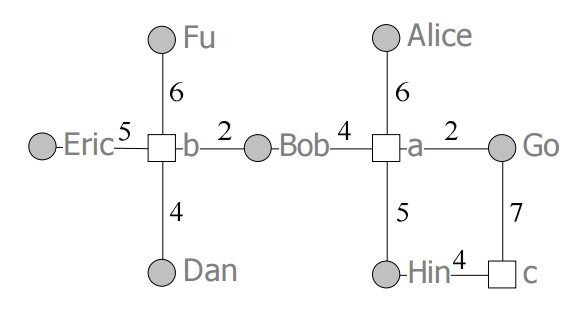
\includegraphics[scale=0.5]{network}
\caption{A sample of a developer-module network for a small project of seven developers and three files. This network diagram is from \cite{pingzer:networks}.}
\label{fig:network}
\end{figure}

Figure \ref{fig:network} represents a developer-contribution for a small project consisting of three files and seven developers. In it, notice that all edges connect developers and files together and that each edge is weighed with the number of commits that developer made to the file. For example, the developer actor named "Hin" is fairly active in the network, they contribute five times to file \textit{a} and four times to file \textit{c}.  Further, file \textit{b} is a highly central file in the network as it is contributed to by "Fu", "Eric", "Dan", and "Bob".

\subsection{Network Centrality}
In the field of social network analysis, network centrality refers to metrics that describe the most important or powerful actors in a social network. Since the definition of a "powerful" actor is fairly arbitrary, there are many different types of network centrality metrics that can be used to quantify this concept \cite{hanneman:network_methods}. For this project, we use betweenness, closeness, and degree centrality in our study as they fit well with the developer-module network and are easy to compute with the information available to us from GitHub.

For the betweenness centrality metric, basic Freeman betweenness centrality is utilized in our study. For each node, Freeman betweenness centrality can be defined as the number of shortest paths in a graph that pass through that node \cite{hanneman:network_methods}. By definition, this notion makes sense since more powerful actors in a network are more likely to introduce other actors to each other. This formula can be generalized as follows:
\[Betweenness(a) = \sum_{s \neq a \neq f} \frac{Short_{s, f}(a)}{Short_{s, f}}\] 
This formula essentially states that the betweenness for an actor is proportion of all shortest paths for each pair of nodes that pass through it. As such, for the purposes of this project, we hypothesize that file actors with a higher betweenness centrality will be more \textit{bug prone} since they are more central to the development of the project.

For closeness centrality, our study uses the path distance version of the metric to calculate the metric. The closeness centrality of an actor in a graph is a measure of how central that actor is to other actors \cite{hanneman:network_methods}. Essentially, the value of closeness centrality for a node in a graph is the inverse of the sum of all shortest paths from that node to all other nodes. as such, the formula for closeness centrality for some node \textit{a} is:
\[Closeness(a) = \frac{1}{\sum_{n = 0}^{N}Short_{s, n}}\]
Essentially, the more central a node is to all other nodes, the smaller the value of the shortest paths and the higher the closeness centrality. As such, we hypothesize that file actors with a higher closeness centrality value are more likely to be \textit{bug-prone} as they are more central among the developers in the network.

Finally, for degree centrality, we utilize Freeman degree centrality in the study. This metric can be defined as the degree of each actor in the graph \cite{hanneman:network_methods}. For instance, looking at figure \ref{fig:network}, the file \textit{a} has a Freeman degree centrality of four. This type of centrality ignores the weights of the edges. For this type of centrality we hypothesize that files with a high degree centrality are likely to be fragmented and more \textit{bug-prone} This is because in files with high degree centrality, there are a greater number of individuals modifying the file during development of the project. This means that developers will have to deal with other developers' code and may be changing components that they do not fully understand.
 
%%%%%%%%%%%%%%%%%%%%%%%%%%%%%%%%%%%%%%%%%%%%%%%%%%%%%%%%%
% Body of Paper
%%%%%%%%%%%%%%%%%%%%%%%%%%%%%%%%%%%%%%%%%%%%%%%%%%%%%%%%%
\section{Empirical Study with Boa}
\label{study}
To validate the findings of previous research that deals with social networks and failure prediction \cite{pingzer:networks} and to achieve the research questions stated in the previous section, we conducted a study that aimed to construct developer-module networks for several large, open-source projects on GitHub. This study used these developer-module networks to compute centrality metrics for each project and teste whether these metrics are correlated with the number of commits and bug fixes in a project. Further, we tested whether network centrality metrics can be used to predict \textit{bug-prone} files. The remainder of this section describes the dataset and methodology used as well as the software tool developed for the study.

\subsection{Dataset}
As the number of research projects that study GitHub repositories increases, several different solutions have emerged which allow for rapid access to open-source project data \cite{Kalliamvakou:GitHub}. First introduced in 2013 by researchers at Iowa State, one project called Boa has developed a domain specific language (DSL) that allows for access to numerous software version control repositories such as GitHub and SurgeForge in a standardized way \cite{Dyer:Boa}. The  Boa DSL is advantageous as it is simple to use and has the ability to pull aggregate information from several thousand projects over the course of several minutes. In addition to the Boa's DSL, the project also contains a large dataset of GitHub repositories from September, 2015 that can be accessed through Boa queries. 

Due to the inherent limitations of the GitHub API such as rate limits and poorly defined schemas, this study does not access project data directly from GitHub. Rather, this study uses the Boa project's query language and dataset to collect project information for use in constructing developer-module networks. Boa is advantageous over other GitHub datsets such as \textit{GHTorrent} due to its well defined schema, simple DSL, and flexible Java application programmer interface (API). Further, since the current Boa dataset includes projects from September 2015, this study will be able to access the data from recent versions of many different open-source projects. While it may appear that Boa is a great fit for use in this project, several limitations were encountered during its use in this study. While not overly problematic, these limitations are discussed thoroughly in section \ref{future_work} of this paper.

By using Boa in this study, we developed a Boa query called \textit{project search} that allows us to search its dataset for projects based on the number of contributors, files, and ratio of regular commits to bug fix commits. Further, we developed a Boa query called \textit{contribution data} that is able to pull all data required to build the contribution network. Specifically, this query returns a list of all files in the project, a list of contributors, and a list of files changed by each commit. These two scripts allow for us to easily download data that can be used to construct the developer-module networks used in the study. 

Due to the sheer size of the Boa dataset and query execution time for Boa queries, project data used in this study was cached locally in a database for quick future access. Since the \textit{contribution data} query used in this study takes, on average, several minutes to complete regardless of project size, caching results ensured contribution networks could be rapidly rebuilt. Further, since these contribution networks were built multiple times over the course of the study, we wanted to limit the number of queries submitted to the Boa project servers. Since this service is a privilege open to all researchers, we wanted to avoid abusing their query service. The schema of the database used to locally cache projects is discussed in detail in section \ref{software_tool}.

\subsection{Methodology}
\label{methodology}
\subsubsection{Developer-Module Networks \& Centrality}
\label{developer_networks}
Before we could answer both research questions stated in the previous section, we first had to transform the data obtained from the \textit{contribution data} Boa query for each project into a custom developer-module network. For the purposes of this study, developer module networks can be defined as specialized graphs of the form \(G = (D, F, E)\) where \(D\) are the developers, \(F\) are the files, and \(E\) are the commits from \(D \to F\). As such, we constructed a standard graph using the formal definition of developer-module networks for each project queried. For each of the actors, we stored pertinent data such as the actor's number of commits and bug fixes. Further, since each developer could have multiple commits to a file, each of the ties in \(E\) were weighted with the number of commits that the developer made to each file. Based on the output format of the \textit{contribution data} query, we were able to analyze the output file and extract it into graph format fairly easily.

Importantly, since this study aimed to predict whether files were \textit{bug-prone}, we had to develop a definition of \textit{bug-proneness} using data available from Boa. Since the Boa dataset does not store GitHub Issue data we opted to count the number of commits to each file that fixed bugs. We coin this type of commit as a \textit{bug fix commit}. To determine whether a commit is aimed at fixing a bug, we first developed a regular expression function in Boa that looked for specific keywords in the commit log such as "fix" or "revision". After a few unsuccessful tries using our custom function, we discovered that Boa contains a method called \textbf{isfixingrevision(...)} that returns true if a commit was used to fix a bug. As such, the Boa query \textit{contribution data} returns the number of commits and bug fix commits for each file. With this data, we are then able to denote \textit{bug-proneness} of a file to be,
\[BugProne(f) = \begin{cases} 1, \frac{BugFixes(f)}{Commits(f)} > Median(\frac{BugFixes}{Commits}) 
\\\\0, \frac{BugFixes(f)}{Commits(f)} \leq Median(\frac{BugFixes}{Commits})
\end{cases}\]
This formula states that if the proportion of bug fixes to commits for a file is greater than the median of bug fixes to commits for that project, the file will be considered to be \textit{bug-prone}. Otherwise, the file is \textit{non-bug-prone}. 

In addition to constructing the developer-module networks, the network centrality metrics needed to be computed before the research questions could be answered. As stated in the previous section, we used the betweenness, closeness, and degree centrality metrics for this study. These metrics are each computed for each file actor in the network and stored for later use.

\subsubsection{Spearman Correlations}
Once the developer-module networks were constructed and network centrality metrics were computed, we could answer our research questions. First to determine whether the betweenness, closeness, and degree centralities correlated with the number of commits and bug fix commits for each project, we calculated the Spearman correlations between each metric for each project. The metrics we used in the Spearman correlation test are each type of network centrality, the number of commits, and number of bug fix commits. Since we have five different metrics to test and one calculation requires two different sets of metrics, fifteen different Spearman correlation values needed to be calculated. The input into the Spearman correlation function is a list of values for each metric being tested that corresponds to each file in the network. The output of the Spearman correlation function is a value between -1 and 1 inclusive that indicates the strength of the correlation. Once we calculated the Spearman correlation for all the metrics, we performed a Paired T-Test to determine whether the confidence level fell within a threshold of 0.01 for each calculation.

\subsubsection{Logistical Regression}
To answer the second research question of whether developer-module networks could be used to predict failures, we perform logistic regression for each project. The purpose of this test is to develop logistical models from centrality metrics that will be used to predict whether files in the project are \textit{bug-prone} files. As defined in section \ref{developer_networks}, the notion of \textit{bug-prone} and \textit{non-bug-prone} files are important here to allow us to build a model using logistical regression and to validate the results of the predictive model on a testing set of files.

Before the regression could be performed, we used the definition of \textit{bug-prone} and \textit{non-bug-prone} to assign each file a label of 0 or 1. Files that were \textit{bug-prone} were assigned a label of 1 and files that were \textit{non-bug-prone} were assigned a label of 0. In addition to the label, each file being inputted into the logistical regression function required a dense vector of features that contained the three centrality metrics calculated for that file. Since the values of each of the three centrality metrics had different ranges of values, each list of centrality metrics for that project was independently standardized through calculation of the z-score. This means that each centrality metric set had a mean of 0 and standard deviation of 1 \cite{hanneman:network_methods}.  This standardization allows for nicer probabilities to be outputted for each of the files in the testing set. Further, due to the normalization, each of the predicted scores outputted from the logistical regression function will now have a score that can be positive or negative. As such, we decided to set a threshold of 0 such that positive scores calculated from the predictive model would denote a \textit{bug-prone} file and negative scores would be predictions for a \textit{non-bug-prone} file.

After formatting the input, the logistic regression is run 100 times for each project using a 60:40 split. Therefore, for each run of the logistic regression test, 60\% of the project is used to train the model and 40\% are used for predictions. Further, the purpose of running the logistic regression function 100 times per project is to ensure that a single split configuration will overly influence the precision and recall results of the project. Once run 100 times, the precision and recall are calculated from each of the predictions for each of the runs. Finally, the mean and median values are computed using all the outputted values to deliver a final precision and recall value.

\subsection{Software Tool}
\label{software_tool}
Since the methodology described in \ref{methodology} needed to be performed for a variety of different projects, a software tool called \textbf{NetworkMine} was developed that automates the methodology of the entire study. Written in Java and Scala, the NetworkMine tool is comprised of two independent but connected components; the Boa miner and the social network builder. The Boa miner is responsible for pulling all project data from the Boa website for a specific list of projects. The social network builder is responsible for constructing the developer-module network, calculating all relevant metrics, and running the Spearman correlation and logistical regression functions on each network. The purpose of this division in components is important because, in future iterations of the tool, Boa could be swapped for different GitHub mining repositories such as \textit{GHTorrent}. The remainder of this section will explain the two sections of the tool in detail.

\subsubsection{Boa Miner}
The Boa miner component is responsible for pulling project data from Boa's servers into a local SQLite3 database. The tool allows for users to search for projects based on the number of contributors and files. Further, users can download projects from the small, medium and large GitHub datasets hosted by the Boa project. Once a list of projects is found that match a user's desired search parameters, the user can download any number of those projects. Figure \ref{fig:miner} shows a screenshot of the tool allowing users to select projects to download. In this figure, users can select multiple items in the list to download in one run. Each project selected will execute its own Boa query that will pull all relevant project data. The tool is implemented with a graphical user interface to allow for ease of use.

\begin{figure}
\centering
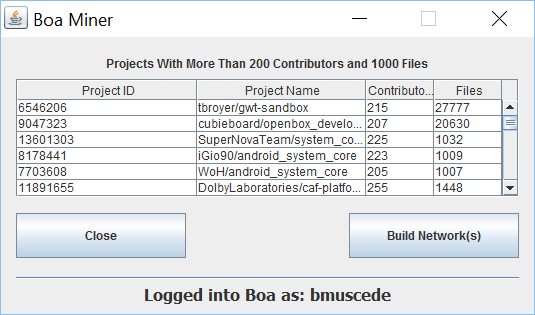
\includegraphics[scale=0.95]{boa_miner}
\caption{The Boa miner tool showing all projects in the Boa dataset that have over 200 contributors and 1,000 files.}
\label{fig:miner}
\end{figure}

The Boa miner component is written in Java and requires the SQLite JDBC driver library and Boa API developed by Iowa State. It uses a modified version of both the \textit{project search} and \textit{contribution data} queries to find projects and download contribution network data. The modified versions of these queries contain a special "placeholder" tag that allows the Boa miner to insert user defined parameters into the query. Due to limitations of the Boa API, the queries are executed on Boa's servers in a concurrent fashion. This makes the tool slow when downloading multiple projects. Concurrency issues isolated to the Boa API prevented us from integrating multithreading in this tool.  

\subsubsection{Local Database}
The local database for this project is a simple SQLite database stored in a user defined directory. The database contains five different tables which allow for multiple projects to be stored at once. A simple entity-relationship (ER) diagram of the database is shown in figure \ref{fig:er}. For the two relationships in the ER diagram that have a many to many multiplicity, an additional table was built to express it. A schema file is included with the tool to allow for the database to be rebuilt from scratch.

\begin{figure}
\centering
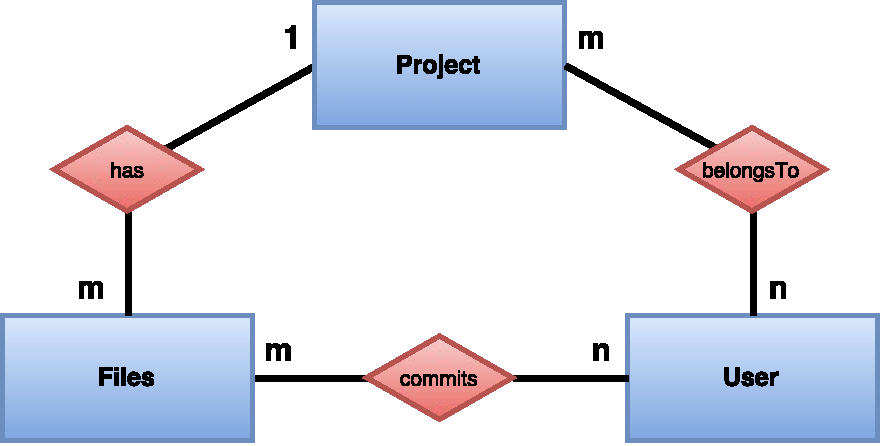
\includegraphics[scale=0.5]{er_database}
\caption{A simple entity-relationship diagram demonstrating the relationship of the project, user, and file tables. The multiplicity for each relationship is shown.}
\label{fig:er}
\end{figure}

\subsubsection{Social Network Builder}
The social network builder component carries out the brunt of the methodology. Using the project data downloaded from the Boa miner component, the social network builder constructs a developer-module network for a specified project and then computes the betweenness, closeness, and degree centrality metrics for that graph. Once complete, the user is then able to see the results of the Spearman correlation test for each social network metric and the results of the logistic regression analysis conducted on the graph. Unlike the Boa miner component, this component does not have a graphical user interface and is simply accessed via the command line. The output of the program is a comma-separated values (CSV) file that contains the results of the Spearman correlation and logistic regression functions for all specified projects. 

Importantly, the social network builder relies on several open-source libraries including Java Universal Network/Graph Framework (JUNG) and Apache Spark. JUNG is used to develop the graph and compute centrality metrics. Apache Spark, while normally used as a cluster computing framework, is used to perform the logistic regression using the MLLib machine learning library. This component is mostly written in Java but employs Scala for the logistic regression functions due to Scala's verbosity. The tool has many options that can be set including the number of projects to analyze from the database, the output file locations, the number of iterations performed for the logistic regression, and the percentage split of the testing and training sets. 

\section{Results}
\label{results}
This section describes the results that were obtained after running the \textbf{NetworkMine} tool across a collection of projects stored in the Boa dataset. The results described here were obtained through meticulously following the methodology described in the previous section. Here, we described the projects that we selected for use, the results of the Spearman correlation analysis, and the logistic regression analysis.

\subsection{Selected Projects}
While the Boa dataset has a large number of GitHub software projects that could be used in this study, we decided to limit our scope by focusing on a subset of these projects. While this project aims to test whether developer-module networks are able to predict failures over a large number of GitHub projects, too many projects would take far too long to compute and also dilute the results presented in this paper. As such, we decided to select fifteen large projects that would form a good representative sample. Fifteen is a good value since it will allow us to test our hypothesis on a variety of different projects to eliminate the possibility of chance while not being too many. Further, while we wanted larger projects with many files and contributors, we decided not to select the top fifteen largest projects from the Boa dataset since many tended to be divergent forks of the Android project. Including projects of a similar nature would result in duplicate results that could spoil the conclusion.

%Table for the statistics of the project.
\begin{table}
\centering
\caption{Selected Project Statistics}
\label{tab:proj_stats}
\begin{tabular}{|c|c|c|c|c|} \hline
&\textbf{Users}&\textbf{Files}&\textbf{Commits}&\textbf{Bug Fixes}\\ \hline
\textit{Average}&190.20&3268.47&27.30&4.69\\ \hline
\textit{Max}&308&6683&4486&1472\\ \hline
\textit{Min}&102&1448&1&0\\ \hline
\end{tabular}
\end{table}

Based on all these considerations, we selected fifteen projects that each had over 150 contributors and 1,000 files that were from a variety of different software domains. Table \ref{tab:proj_stats} shows the several statistics pertaining to the project set that was used. The project dataset can be divided into four different domains; Android tools, programming development software, programming frameworks, and other software. Android tools can be defined as Android operating system components or applications developed by members of the Android open-source community. Programming development software is defined as tools that aid programming such as integrated development environments or task trackers. Programming frameworks are protocols, tools, or libraries that can be used during development. Lastly, other software is simply several software projects that do not fit the other three categories. Of these domains, 4 of the projects used are part of the Android tools domain, 4 are programming development software, 4 are programming frameworks. and 3 are miscellaneous software projects.

\subsection{Spearman Correlation}
Similar to Pinzger et al., for each project that we tested, we computed the Spearman correlation between each of the metrics to determine whether there was a correlation between each of these metrics. In it, values below -0.5 and above 0.5 are denoted to be correlated and values below -0.7 and above 0.7 and above are denoted to be strongly correlated components. Table \ref{tab:spearman} shows the mean results of the Spearman correlation test computed for each of the five metrics that were used in the study. We present the mean across all projects since it is infeasible to display the results from all of the projects. However, each correlation calculated in each project is significant at the 0.01 level. This was calculated through the use of a Paired T-Test.

%Table for general Spearman correlations.
\begin{table*}
\centering
\caption{Mean Spearman correlations across all projects in the study. Values above 0.5 denote a positive correlation and values above 0.7 denote a strong positive correlation. Each correlation for all projects is significant at the 0.01 level (2-tailed).}
\label{tab:spearman}
\begin{tabular}{|c|c|c|c|c|c|c|} \hline
&\textbf{Commits}&\textbf{Bug Fixes}&\textbf{Betweenness}&\textbf{Closeness}&\textbf{Degree}\\ \hline
\textbf{Commits}&1.00&0.811&0.507&0.173&0.852\\ \hline
\textbf{Bug Fixes}&&1.00&0.453&0.213&0.750\\ \hline
\textbf{Betweenness}&&&1.00&0.627&0.723\\ \hline
\textbf{Closeness}&&&&1.00&0.459\\ \hline
\textbf{Degree}&&&&&1.00\\ \hline
\end{tabular}
\end{table*}

Despite the mean, some projects correlated strongly with bug fixes and commit numbers for all centrality metrics while others did not. Table \ref{tab:spearman_diff} shows the difference in correlation values between the Spearman correlations for the \textit{Caf-Platform} (values in black) and \textit{Dropwizard} projects (values in red). Some of the correlations are close to 0 indicating that the values have no correlation at all. This lack of a positive correlation between bug fixes and the centrality metrics indicates that logistic regression may not work well at predicting bug-prone files for this project. Despite this, on average, the number of bug fixes tends to be positively correlated with all three centralities.

%Table for specific projects.
\begin{table*}
\centering
\caption{Spearman correlation values for the each network metric in the \textit{Caf-Platform} project (values are on left and in black) and the \textit{Dropwizard} project (values are on right and in red) Each correlation for all projects is significant at the 0.01 level (2-tailed).}
\label{tab:spearman_diff}
\begin{tabular}{|c|c|c|c|c|c|c|} \hline
&\textbf{Commits}&\textbf{Bug Fixes}&\textbf{Betweenness}&\textbf{Closeness}&\textbf{Degree}\\ \hline
\textbf{Commits}&1.00 / {\color{red} 1.00}&0.927 / {\color{red} 0.680}&0.802 / {\color{red} 0.251}&0.870 / {\color{red} -0.281}&0.971 / {\color{red} 0.737}\\ \hline
\textbf{Bug Fixes}&&1.00 / {\color{red} 1.00}&0.782 / {\color{red} 0.093}&0.821 / {\color{red} -0.133}&0.933 / {\color{red} 0.529}\\ \hline
\textbf{Betweenness}&&&1.00 / {\color{red} 1.00}&0.898 / {\color{red} 0.616}&0.867 / {\color{red} 0.675}\\ \hline
\textbf{Closeness}&&&&1.00 / {\color{red} 1.00}&0.926 / {\color{red} 0.332}\\ \hline
\textbf{Degree}&&&&&1.00 / {\color{red} 1.00}\\ \hline
\end{tabular}
\end{table*}

Based on both tables presented here, there are some interesting conclusions that can be gained. First, not all the projects had failure or commits correlate highly with some of the three centrality metrics. This is especially evident when looking at the closeness centrality metric in Table \ref{tab:spearman} as its value indicates that it failed to correlate well with the number of bug fixes and commits metrics for all projects. Despite this, the degree centrality of all projects tended to be highly correlated with the commits and bug fixes. Overall, the results from this portion of the study indicate that these centrality metrics tend to be decently correlated with commits and bug fixes.

\subsection{Logistic Regression}
After computing the Spearman correlations, logistic regression for each developer-module network was conducted. In the regression, we set \textit{bug-prone} files with a label of \textbf{1.0} and \textit{non-bug-prone} files with a label of \textbf{0.0}. Each feature label was accompanied by a dense vector of the standardized value of the three centrality values computed for that file. To ensure each project was thoroughly tested, logistic regression was performed 100 times for each project and 60\% of the files in the graph were randomly divided into the training set and 40\% into the testing set. In the output from the logistic regression test, was a collection of file labels with a predicted probability score between -1 and 1. We selected 0 as the cutoff point in the output score that divides \textit{non-bug-prone} and \textit{bug-prone}.

%Table for specific projects.
\begin{table}
\centering
\caption{Precision and recall values for the top three and bottom three projects. Average results for all projects are included in the bottom.}
\label{tab:regression}
\begin{tabular}{|c|c|c|c|c|c|c|c|c|} \hline
\textbf{Top Projects}&&\textbf{Precision}&\textbf{Recall}\\ \hline

\multirow{2}{*}{Gerrit}&Mean&0.797&0.951\\ \cline{2-4}
&Median&0.797&0.951\\ \hline
\multirow{2}{*}{Caf-Platform}&Mean&0.753&0.816\\ \cline{2-4}
&Median&0.753&0.813\\ \hline
\multirow{2}{*}{System Core (Android)}&Mean&0.715&0.815\\ \cline{2-4}
&Median&0.740&0.818\\ \hline
\end{tabular}
\newline
\vspace*{0.1 cm}
\newline
\begin{tabular}{|c|c|c|c|c|c|c|c|c|} \hline
\textbf{Bottom Projects}&&\textbf{Precision}&\textbf{Recall}\\ \hline

\multirow{2}{*}{Gem5}&Mean&0.568&0.861\\ \cline{2-4}
&Median&0.546&0.880\\ \hline
\multirow{2}{*}{PhoneGap-Plugins}&Mean&0.911&0.537\\ \cline{2-4}
&Median&0.911&0.537\\ \hline
\multirow{2}{*}{Google Closure Comp. }
&Mean&0.999&0.647\\ \cline{2-4}
&Median&1.000&0.648\\ \hline
\end{tabular}
\newline
\vspace*{0.1 cm}
\newline
\begin{tabular}{|c|c|c|} \hline
&\textbf{Precision}&\textbf{Recall}\\ \hline
Mean&0.756&0.765\\ \hline
Median&0.730&0.781\\ \hline
\end{tabular}
\end{table}

Table \ref{tab:regression} shows several descriptive metrics for the results of the logistic regression for the top four and bottom four projects. In it, the number of iterations for the logistical regression for each project displayed has been compressed through calculations of the mean and median. Further, the table presents the mean and median precision and recall across all iterations in all projects. 

The results obtained from the use of logistic regression are encouraging. While several projects in the bottom four tend to have either very low precision or recall, the projects with the top precision and recall values indicate that centrality metrics can possibly be used as valid bug predictors. For instance, since the Gerrit project has a precision and recall values of over 80\%, there are few false positives and negatives being included in the predictions. Further, many of the projects tested have higher recall values compared to precision. This is desirable in the scope of failure prediction since having false positives included in the bug predictions is less detrimental than having false negatives. For example, if these predictions are used to decide which files to closely inspect files for bugs, false positives will simply mean that more files will need to be inspected. On the other hand, false negatives will mean that certain bug-prone files will miss the closer inspection.

\begin{figure}
\centering
\vspace*{-3mm}
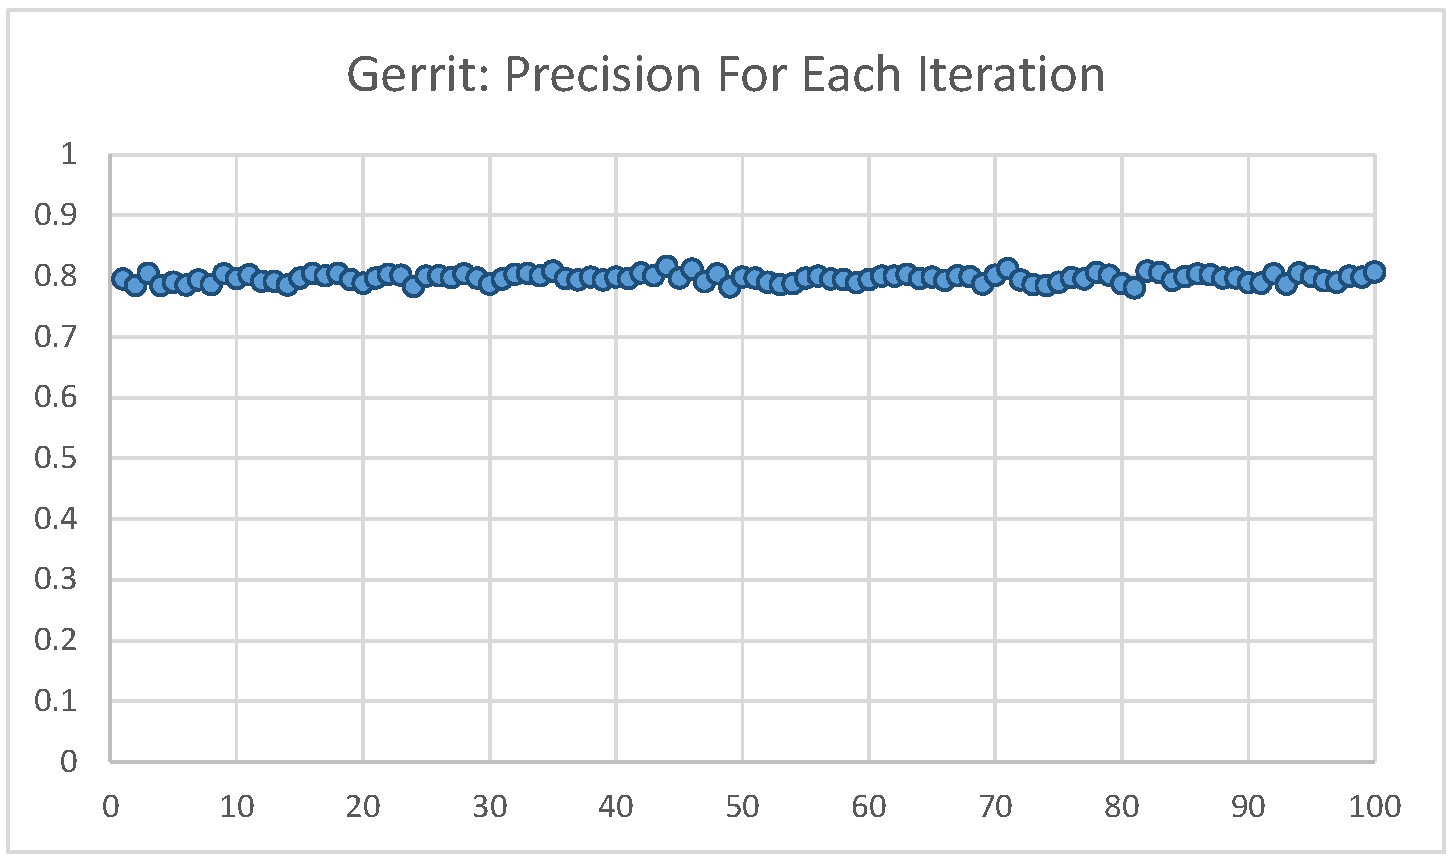
\includegraphics[scale=0.35]{gerrit_precision}
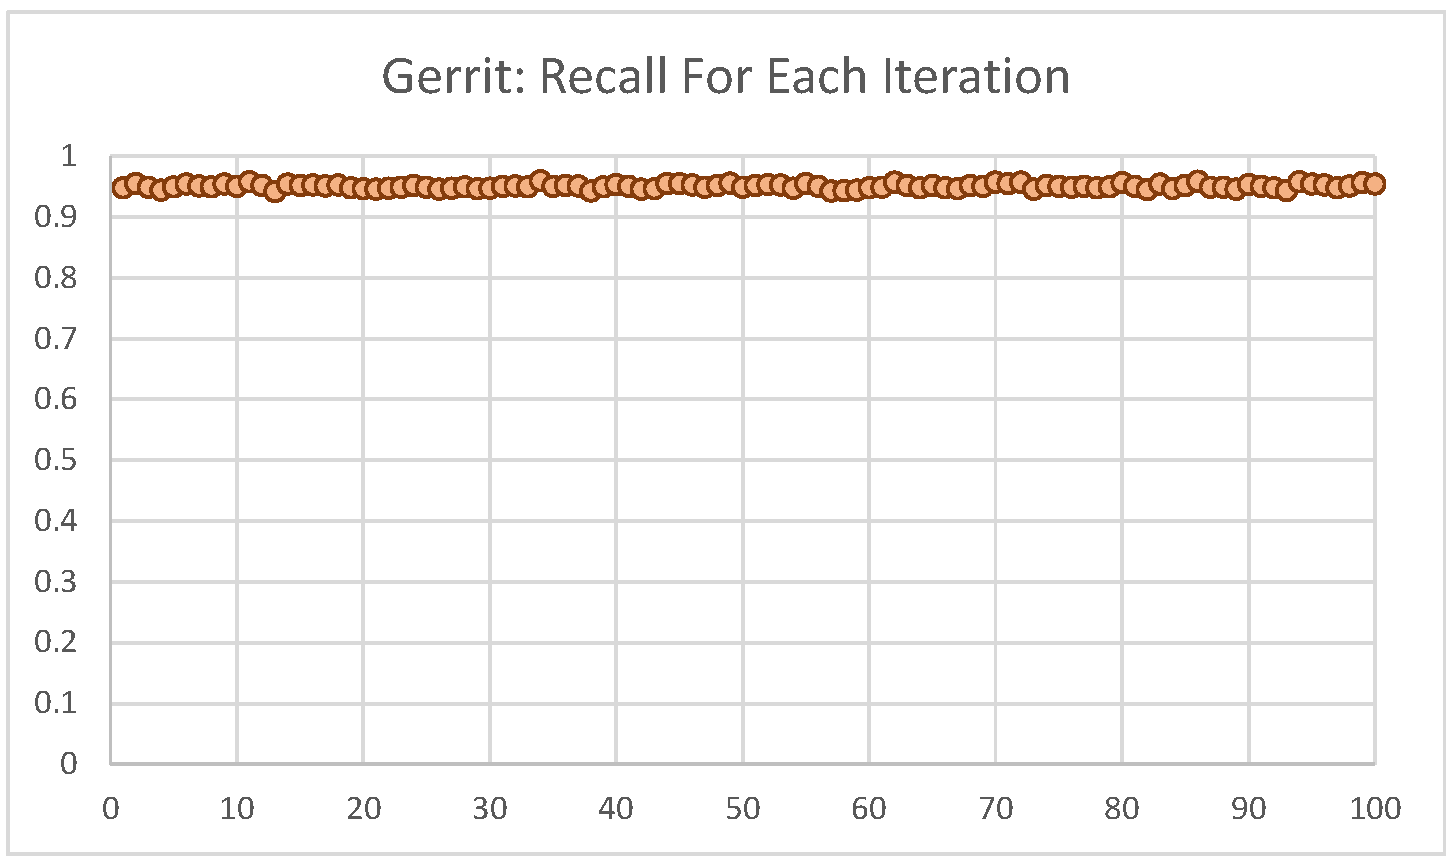
\includegraphics[scale=0.35]{gerrit_recall}
\caption{The precision and recall values for each iteration of the 
logistic regression test for the Gerrit project.}
\label{graph:prec_rec}
\vspace*{-3mm}
\end{figure}

Figure \ref{graph:prec_rec} shows a scatterplot of the precision and recall values for the Caf-Platform project. Since most of the runs of the logistic regression function present similar precision and recall values, the standard deviation of the data is low. This further validates the results as it demonstrates that, even with different splits of the input graph, the logistic regression function is able to predict the precision and recall fairly well.

\section{Future Work}
\label{future_work}
While the results of the study are encouraging, we have identified several areas of work that allow for further research to investigate and improve the \textbf{NetworkMine} tool. While these areas of research expand upon the methodology presented in this paper, they do not invalidate or introduce major threats to validity for the study.

In our study, we used three different types of network centrality metrics; betweenness centrality, closeness centrality and degree centrality. While the study was successful using these metrics, computing further centrality metrics may strengthen the predictions made by the logistic regression function. For instance, in this study, we define degree centrality to be the number of ties that an actor has to other actors in the graph. While this type of degree centrality, known as Freeman degree centrality, is commonly used by social network researchers, there is another type of degree centrality called Bonacich's power. Bonacich's power measures the power actors have over other actors in the network. The idea is that actors that have ties to only a few other actors are considered more powerful since they are more likely to influence their neighbours \cite{hanneman:network_methods}. Simply put, it challenges the notion that actors that are more central are most powerful. It is hypothesized that using these additional centrality metrics is likely to increase the predictive power of the logistic models.

Another improvement to the methodology proposed in this study is to perform network preprocessing before calculating the Spearman correlations and performing the logistic regression function. Used in related work \cite{pingzer:networks}, this preprocessing could be used to improve the quality of the graph and remove any unusual actors or ties that might introduce faulty results. There are many different examples of projects that benefit from this preprocessing stage. For instance, pruning files from the network that are not source code would be beneficial. This includes files such as \textit{.gitignore}, image files, or even GitHub markdown files. Of course, additional research needs to be conducted to determine the feasibility and effectiveness of pruning the graph in this way. Another preprocessing operation that might benefit the results would be removing user actors that have ties to the majority of file actors in the graph. These user actors might be automated bots that add copyright headers to each file or users that simply are tasked with formatting the code style of the project's code. It would be detrimental to keep these users in the graph and have them influence centrality scores.

Finally, there are several proposed improvements to the NetworkMine tool. First, while Boa has been an asset for this project, it would be beneficial to allow users to pull from different GitHub datasets such as \textit{GHTorrent}. This would allow users to have a larger choice of projects to select. Another motivation for this is that, while the Boa project has a large dataset and provides a powerful DSL for powerful query expressions, our project does not use Boa for its intended purpose. The Boa project is largely tasked at providing researchers with a feasible way to compute certain statistics across all projects in a dataset \cite{Dyer:Boa}. As such, the queries developed in this project still iterate through every single project in the dataset despite being targeted for a specific project. This means that Boa queries that would download network data for one project would take just as long as queries designed to target all projects. In addition to Boa, we would like to increase the functionality of this tool so that it has a graphical user interface and can visualize the developer-module networks. 

%%%%%%%%%%%%%%%%%%%%%%%%%%%%%%%%%%%%%%%%%%%%%%%%%%%%%%%%%
% Conclusion
%%%%%%%%%%%%%%%%%%%%%%%%%%%%%%%%%%%%%%%%%%%%%%%%%%%%%%%%%
\section{Conclusion}
In this paper, we presented a study that analyzed the developer-module networks for fifteen different open-source projects on GitHub. The study showed that, on average across all projects, betweenness and degree centrality are correlated with the number of commits and bug fixes. Further, the project demonstrated that for some projects, \textit{bug-prone} files could be predicted with high precision and recall through the use of network centrality. In addition, we started development of a tool called \textbf{NetworkMine} that enables users to emulate the methodology presented in this paper on any desired GitHub project. In the future, we aim to expand the functionality of the NetworkMine tool to allow for different project datasets and to implement developer-module network visualization features.

%%%%%%%%%%%%%%%%%%%%%%%%%%%%%%%%%%%%%%%%%%%%%%%%%%%%%%%%%
% Bibligography.
%%%%%%%%%%%%%%%%%%%%%%%%%%%%%%%%%%%%%%%%%%%%%%%%%%%%%%%%%
\bibliographystyle{IEEEtran}
\bibliography{sigproc}

\balancecolumns
\end{document}
